\documentclass[12pt]{article} % for thesis

% \usepackage[top=0.5in, bottom=0.5in, left=0.5in, right=0.5in]{geometry}
% \documentclass[twocolumn,9pt]{article}
\usepackage{spconf}
\usepackage[utf8]{inputenc}
\usepackage{natbib}
\usepackage{graphicx}
\usepackage{stfloats} % for positioning of figure* on the same page
\usepackage{caption}
\usepackage{tikz}
\usepackage[inline]{enumitem}
\usepackage{amsmath}
\usepackage[breaklinks=true,colorlinks=true, allcolors=blue]{hyperref}
\usepackage{breakcites}
\usepackage{microtype}
\usepackage{lipsum}
\usepackage{xcolor}
\usepackage{array}
\usepackage{float}
\usepackage{adjustbox}
\usepackage{listings}
\usepackage{csquotes}
\usepackage{makecell}
\usepackage{pdfpages}
\usepackage{xspace}
\usepackage{tikz}

\usetikzlibrary{positioning,shapes.geometric}

% to do:
% hearing tests
% one other way to present results is grouped by which losses are most appropriate for each situtation

\usepackage{xcolor}
\usepackage[utf8]{inputenc}       % For UTF-8 encoding
\usepackage{listings}
\usepackage{amsmath}              % Optional: for math symbols
\usepackage{anyfontsize}
\usepackage{graphicx} % required for \scalebox

\lstdefinelanguage{Faust}{
    morekeywords={import, process, environment, declare, with, if, else, while, for, int, float, true, false},
    sensitive=true,
    morecomment=[l]{//}, % Line comment
    morecomment=[s]{/*}{*/}, % Block comment
    morestring=[b]", % Strings
}

% Customize the appearance of the code
\lstset{
    language=Faust,
    backgroundcolor=\color{lightgray!20},
    % basicstyle=\ttfamily\small,
    basicstyle=\fontsize{8pt}{9pt}\selectfont\ttfamily,
    keywordstyle=\color{blue}\bfseries,
    stringstyle=\color{orange},
    commentstyle=\color{green}\itshape,
    showstringspaces=false,
    % numbers=left,
    % numberstyle=\tiny,
    frame=single,
    breaklines=true,
      % basicstyle=\ttfamily,
  % literate={\delta}{{\(\delta\)}},
}


\captionsetup[lstlisting]{justification=centering, singlelinecheck=false}
\providecommand{\gls}[1]{#1}
\newcommand{\highlight}[1]{\textcolor[RGB]{00,150,00}{#1}}
\newcommand{\todo}[1]{\textcolor{red}{#1}}

\newcommand{\SIMSESpec}{\texttt{SIMSE\_Spec}\xspace}
\newcommand{\LoneSpec}{\texttt{L1\_Spec}\xspace}
\newcommand{\JTFS}{\texttt{JTFS}\xspace}
\newcommand{\DTWEnv}{\texttt{DTW\_Envelope}\xspace}
\newcommand{\OutDomain}{\textbf{Out-of-Domain Generation}\xspace}
\newcommand{\LossSelect}{\textbf{Loss Selection}}
\newcommand{\SynthSelect}{\textbf{Synthesis Selection}}
\newcommand{\PeriodicLoss}{\textbf{Periodic Loss}}

\newcommand{\BPNoise}{\textbf{BP-Noise}\xspace}
\newcommand{\BPSaw}{\textbf{BP-Saw}\xspace}
\newcommand{\AddSineSaw}{\textbf{Add-SineSaw}\xspace}
\newcommand{\AmpMod}{\textbf{Noise-AM}\xspace}
\newcommand{\FMMod}{\textbf{SineSaw-AM}\xspace}
\newcommand{\FMModvtwo}{\textbf{SineSine-AM}\xspace}
\newcommand{\PitchBendUp}{\textbf{PitchBend-Up}\xspace}

\title{Selecting Loss Functions for Out-of-Domain Sound-Matching}
\begin{document}

\name{Amir Salimi, Abram Hindle, Osmar R. Za{\"i}ane}
\address{University of Alberta}

\maketitle

%     Despite their critical role in sound-matching, the performance of different sound-similarity measures (or loss functions) under different circumstances has rarely been a topic of research. Should we be looking for a global sound-similarity measure, or is the choice of loss function a creative decision, much like the selection of a synthesizer?

\begin{abstract}
 Out-of-domain sound-matching is the task of automatically programming a synthesizer towards a sound that it cannot accurately replicate. While this approach to sound-matching is far better suited for practical applications to design, it has rarely been explored. Measuring performance in out-of-domain sound-matching is a difficult task due to the subjective experience of sound, open-set recognition, characteristics of interest, et cetera. In addition, despite their critical role in sound-matching, the performance of different sound-similarity measures (or loss functions) under different circumstances has rarely been a topic of research. Should we be looking for a global sound-similarity measure, or is the choice of loss function a creative decision, much like the selection of a synthesizer?
 Here we present a series of differentiable out-of-domain sound-matching scenarios using four loss functions and various synthesizers. The experiments here are designed such that differences in parameters (whether all parameters or a subset) are well suited for measuring performance in sound-matching. The out-of-domain experiments here showcase the characteristics of the different loss functions, and confirm that their success is highly dependent on the method of synthesis and the target sound. 
\end{abstract}





\section{Performance Measures}
Manual sound-design is a feedback loop built on the designer hearing an output and measuring the similarity of what is currently generated versus what they would like to hear. This subjective, internal measurement of sound qualities is impossible to recreate between people with similar tastes, let alone digitally. Over the years, many automatic performance measure have been used in previous work, but the generality of such results from such experiments have generally viewed with a large degree of skepticism~\todo{cite}. This is because such experiments have largely been conducted in the in-domain setting, where perfect matching between the target and output sounds ($x^t$ and $x_\theta$), or target and output parameters ($\theta^t$ and $\theta$) is possible. In such cases, reaching the value of zero in L1 or MSS difference of the spectrograms of sounds or the L1 difference between the parameters (i.e., P-Loss) has been a common performance measure. 

In OOD experiments, the usual automatic measures of performance are not applicable. While the subtraction of spectrograms (whether L1, L2, or MSS) can show whether or not two sounds are near identical, larger values in these measures does not correlate with larger differenes~\cite{turian2020sorry,vahidi2023mesostructures}. In addition, P-Loss requires identical parameter sets between synthesizers, which by definition cannot be applied in OOD scenarios. 

In this work we use manual listening tests, which are the gold standard for measuring performance in sound-matching. After all, assistance with manual sound-matching is the most common stated goal of previous sound-matching work~\todo{cite}. In addition, we propose partial P-Loss (PPL), as a reasonable automatic measure of sound-matching performance in our experiments, show whether it correlates with manual listening tests. 



\section{methodology}



\begin{figure}[ht]
    \centering
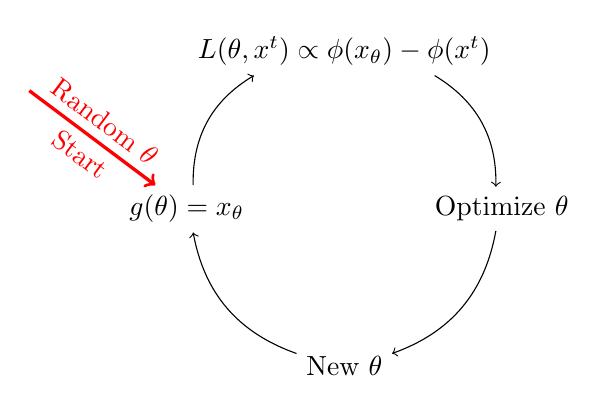
\begin{tikzpicture}[node distance=2cm, auto]

% Nodes
\node (start) [text centered] {\( g(\theta) = x_{\theta} \)};
\node (L) [above of=start, right of=start, text centered] 
    {\( L(\theta, x^t) \propto \phi(x_{\theta}) - \phi(x^t) \)};
\node (optimize) [below of=L, right of=L, text centered] {Optimize $\theta$};
\node (new_theta) [below of=optimize, right of=start, text centered] {New \( \theta \)};

% Highlight and arrow for the start node
\draw[->, very thick, red] (start) ++(-2,1.5) -- (start)
    node[midway, below, align=center, sloped, color=red] {Start}
    node[midway, above, align=center, sloped, color=red] {Random $\theta$};

% Arrows with multi-line labels
\draw[->, bend left] (start) to node[midway, right, align=center] {} (L);
\draw[->, bend left] (L) to node[midway, right, align=center] {} (optimize);
\draw[->, bend left] (optimize) to node[midway, below, align=center] {} (new_theta);
\draw[->, bend left] (new_theta) to node[midway, left, align=center] {} (start);

\end{tikzpicture}

    \caption{ Iterative approach to sound design. Adapted to OOD scenarios~\cite{salimi2025evaluating}.}
    \label{fig:sound_design_loop_iterative}
\end{figure}
\subsection{Problem Setup}

The methodology evaluates loss functions across multiple out-of-domain (OOD) sound-matching scenarios. Each experiment follows the iterative optimization loop in Fig.~\ref{fig:sound_design_loop_iterative}, where a synthesizer $g$ is optimized to imitate a target sound generated by a different synthesizer $g^{t}$. This iterative loop is the adaption of previous work by Salimi \textit{et. al.}~\cite{salimi2025evaluating}.

An \textit{experiment} consists of a complete optimization run: random parameter initialization, 200 steps of gradient-based optimization, and final parameter evaluation. Each experiment is defined by the following components, adapted to OOD settings from previous in-domain work~\cite{salimi2025evaluating,vahidi2023mesostructures}.

\begin{itemize}
    \item $g(\theta)$: A parametric audio synthesizer with parameters $\theta$ producing output $x_{\theta} = g(\theta)$.
    \item $g^{t}(\theta^{t})$: The target synthesizer producing the target sound $x^{t} = g^{t}(\theta^{t})$. OOD conditions require that $g$ and $g^{t}$ differ in structure or parameter ranges such that their output sets do not overlap.
    \item $x_{\theta}$: The imitator’s synthesized audio for parameters $\theta$.
    \item $x^{t}$: The target audio to be imitated.
    \item $\phi(\cdot)$: A feature representation function mapping waveforms into a comparison space.
    \item $L$: A loss function defined as $L(\theta, x^{t}) = d(\phi(x_{\theta}), \phi(x^{t}))$ for some metric $d$.
\end{itemize}

A \textit{scenario} is a group of four experiments---one for each of the four loss functions---performed with the same pair of synthesizers $(g, g^{t})$. Each scenario models a distinct sound-design task, such as matching filter cutoffs, modulation structure, or pitch trajectories, allowing us to evaluate how each loss function behaves under specific forms of OOD mismatch.

\subsection{Loss Functions}
\label{subsec:loss_functions}

We evaluate the same four loss functions used in the previous in-domain study~\cite{salimi2025evaluating}. The functions are summarized below:

\medskip
\noindent\textbf{\LoneSpec:}
This loss computes a pointwise L1 distance between the log-magnitude spectrograms of the imitator and target:
\begin{equation}
    L_{\mathrm{L1}}(\theta, x^{t}) 
    = \left\| STFT (x_{\theta}) - STFT (x^{t}) \right\|_{1}
\end{equation}

The STFT function uses 512 FFT bins, window size of 600 samples, and hop length of 100 samples~\cite{salimi2025evaluating}.

\medskip
\noindent\textbf{\SIMSESpec:}
The scale-invariant mean-squared error (SIMSE). This loss is identical to \LoneSpec, with the exception that it utilizes the SIMSE difference instead of L1.
\begin{equation}
    L_{\mathrm{SIMSE}}(\theta, x^{t}) 
    =  SIMSE( STFT (x_{\theta}) - STFT (x^{t}))
\end{equation}

\medskip
\noindent\textbf{\JTFS:}
The joint time-frequency scattering (JTFS) transform provides a multiresolution representation of temporal and spectral structures of time-series~\cite{vahidi2023mesostructures,anden2015joint}. The loss is defined as:
\begin{equation}
    L_{\mathrm{JTFS}}(\theta, x^{t})
    = 
    \left\|
        \Phi_{\mathrm{JTFS}}(x_{\theta})
        -
        \Phi_{\mathrm{JTFS}}(x^{t})
    \right\|_{2}
\end{equation}
Where $\phi$ is the application of L2 distance metric to the 1-Dimensional JTFS transform provided by Andreux \textit{et. al}~\cite{kymatio,salimi2025evaluating}.

\medskip
\noindent\textbf{\DTWEnv:}
This loss computes a dynamic time-warping (DTW) distance between amplitude envelopes. Since the original DTW function is not differentiable, the soft-DTW distance is used instead~\cite{softdtw_jax}. The envelope of the sound is calculated by taking the STFT, and summing the values of all frequency bins at every time-step~\cite{salimi2025evaluating}.

\begin{equation}
    L_{\mathrm{DTW}}(\theta, x^{t})
    =
    \mathrm{DTW}
    \left(
        \mathrm{Env}(x_{\theta}),
        \mathrm{Env}(x^{t})
    \right).
\end{equation}

\subsection{Evaluation Methods}
\label{subsec:evaluation}
 Evaluations are the scores associated with every experiment, which are later used to determine which loss function is the best performer for which scenario. 

 We have two evaluation methods: human similarity ratings (or likert scores) from a small listening survey, and the automatic partial P-Loss (PPL), which we introduce in this paper as a reasonable measure of performance in OOD settings. 

\subsubsection{Partial P-Loss}
\label{sec:partial_ploss}
In out-of-domain sound-matching, many parameters of the target and imitator synthesizers do not correspond directly; for example, when the target employs a saw oscillator but the imitator uses noise, or when modulation structures differ.  
To evaluate only the aspects of the signal that can meaningfully transfer across domains, we compute a \emph{partial parameter loss} (PPL).  

PPL measures the L1 distance only across the subset of parameters considered perceptually critical for the scenario:
\begin{equation}
\mathrm{PPL} = \| \theta^{(\mathrm{crit})}_t - \hat{\theta}^{(\mathrm{crit})} \|_1,
\end{equation}
where $\theta^{(\mathrm{crit})}$ denotes the target’s critical parameters (e.g., filter cutoffs, modulation rates) and $\hat{\theta}^{(\mathrm{crit})}$ the corresponding recovered parameters of the imitator.  
Parameters with no perceptual or structural correspondence are ignored. 
If done correctly, this can enable a reasonable interpretable comparison across mismatched synthesizers. The PPL for each scenario will be unique, and we will highlight which parameters are used as we describe the scenarios later on.

\subsubsection{Hearing tests}
Hearing tests are the gold standard for measuring performance of sound-matching algorithms. For each scenario, we randomly sample 40 sound-pairs for each loss, and two of the authors listen to the 160 samples in a blinded manner (not knowing which loss was used in the iterative loop). The authors give a Likert score of 1 (not similar at all) to 5 (near identical) to these sound-pairs. These scores are then combined for a total of 320 manual given performance measures for each scenario. 

\subsection{Optimization Loop}
\label{subsec:optimization}


\todo{This contradicts something you've said previous about experiments so decide if you want to keep the definition of experiments the same as before or change it and add trial}A \textit{trial} is defined as one complete 200-step optimization run with a single target sample. An \textit{experiment} consists of 300 independent trials using the same target synthesizer $g^{t}$, imitator synthesizer $g$, and loss function $L$. A \textit{scenario} consists of four experiments that share the same synthesizer pair $(g, g^{t})$ but use different loss functions.

Each trial consists of a 200-iteration gradient-based optimization procedure. Starting from a random initialization $\theta_{0}$, following past work, the imitator synthesizer parameters are updated using the RMSProp optimizer with a fixed learning rate of 0.045~\cite{salimi2025evaluating}.

All synthesizers are implemented in Faust and transpiled into differentiable JAX functions using DawDreamer~\cite{braun2024dac}. 

\subsection{Boostrapping and Ranking Procedures}
\label{subsec:ranking}

We perform all statistical comparisons using bootstrapped performance distributions. For each experiment, the 300 trial-level scores for PPL or 80 scores from survey results are resampled with replacement, and 1000 bootstrapped means are computed. These 1000 values form an empirical distribution that avoids parametric assumptions about the underlying score distribution, and simplifies comparisons between the two performance measures~\cite{chernick2011bootstrap}.

To compare loss functions within a scenario, we apply the nonparametric Scott--Knott procedure (NPSK). For each performance measure, NPSK recursively partitions the bootstrapped distribution to maximize between-group separation while minimizing within-group variance, producing statistically justified ranks without requiring normality~\cite{tantithamthavorn2017mvt,tantithamthavorn2018optimization}. Rank~1 corresponds to the best-performing distribution, with larger ranks indicating worse performance. Ties occur when two or more distributions cannot be statistically distinguished under the NPSK splitting criterion, resulting in equal assigned ranks.

\section{Scenarios and Results}
\subsubsection{Band Pass Matching}
In this scenario, the two synthesizers are the application of band-passing to noise (\BPNoise) and saw waves (\BPSaw). Examples of these programs are given in Listings~\ref{lst:program0} and ~\ref{lst:program0_saw} respectively. Previous observations have shown that with in-domain sound-matching of \BPNoise, the loss functions utilizing spectrogram differences were the best performers, speculating that this due to the clear visibility of filter-cutoffs in a spectrogram~\cite{salimi2025evaluating}. 
 
 Here we use \BPSaw as the target synthesizer, and \BPNoise as the imitator. We define success in sound-matching here as the L1 proximity of the imitator's high and low-pass cutoffs to the corresponding parameters in the target synthesizer. This creates an out-of-domain experiment where P-Loss is an objective measure of success. With this objective, we see that \SIMSESpec is once again the clear best performing loss function.
\begin{table*}[t]
\centering
\small
\setlength{\tabcolsep}{4pt}
\renewcommand{\arraystretch}{1.15}
\resizebox{\textwidth}{!}{%
\begin{tabular}{|l|cc|cc|cc|cc|cc|cc|cc|}
\hline
\textbf{Loss} 
& \multicolumn{2}{|c|}{\textbf{AM: non-overlap}} 
& \multicolumn{2}{c|}{\textbf{AM: sine $\rightarrow$ saw}} 
& \multicolumn{2}{c|}{\textbf{AM: saw $\rightarrow$ sine}} 
& \multicolumn{2}{c|}{\textbf{BP: noise $\rightarrow$ saw}} 
& \multicolumn{2}{c|}{\textbf{Chirp: delayed}} 
& \multicolumn{2}{c|}{\textbf{Chirp: pulsating}} 
& \multicolumn{2}{c|}{\textbf{Chirp: normal}} \\
\cline{2-15}
& \textbf{PP-Loss} & \textbf{Hearing}
& \textbf{PP-Loss} & \textbf{Hearing}
& \textbf{PP-Loss} & \textbf{Hearing}
& \textbf{PP-Loss} & \textbf{Hearing}
& \textbf{PP-Loss} & \textbf{Hearing}
& \textbf{PP-Loss} & \textbf{Hearing}
& \textbf{PP-Loss} & \textbf{Hearing} \\
\hline
SIMSE & 2 & -- & 3 & -- & 2 & -- & 1 & -- & 3 & -- & 2 & -- & 3 & -- \\
L1    & 3 & -- & 4 & -- & 4 & -- & 3 & -- & 4 & -- & 3 & -- & 2 & -- \\
JTFS  & 4 & -- & 2 & -- & 3 & -- & 4 & -- & 1 & -- & 2 & -- & 1 & -- \\
DTW   & 1 & -- & 1 & -- & 1 & -- & 2 & -- & 2 & -- & 1 & -- & 4 & -- \\
\hline
\end{tabular}%
}
\caption{Summary of ranks across seven scenarios using two evaluation measures: bootstrapped PP-Loss and bootstrapped hearing survey ratings. Lower rank indicates better performance.}
\label{tab:scenario_ranks}
\end{table*}


\begin{figure*}[htbp]
  \centering
  \scriptsize

  %-------------------------------------%
  % Left panel
  %-------------------------------------%
  \begin{minipage}{0.48\textwidth}
    \begin{minipage}{0.10\textwidth}
      \raggedleft
      \vspace{0.5cm}
      SIMSE\\[0.6cm]
      L1\\[0.65cm]
      JTFS\\[0.65cm]
      DTW
    \end{minipage}%
    \begin{minipage}{0.87\textwidth}
      \centering
      \includegraphics[width=\linewidth]{images/npsk_ood_P_Loss_3.png}
    \end{minipage}
  \end{minipage}
  \hfill
  %-------------------------------------%
  % Right panel
  %-------------------------------------%
  \begin{minipage}{0.48\textwidth}

    \begin{minipage}{0.87\textwidth}
      \centering
      \includegraphics[width=\linewidth]{images/npsk_ood_likert_3.png}
    \end{minipage}
  \end{minipage}

  \caption{Bootstrapped distributions and NPSK ranks for two band-pass matching setups.}
  \label{fig:npsk_BP_two}
\end{figure*}



\begin{lstlisting}[caption={\BPNoise}, label={lst:program0}, language=Faust,
                  float, floatplacement=!H, xleftmargin=1em, xrightmargin=0.5em, firstnumber=0, aboveskip=0em, belowskip=-1em]
import("stdfaust.lib");
lp_cut = hslider("lp_cut",900,100,5000,5);
hp_cut = hslider("hp_cut",100,1,400,5);
process = no.noise:fi.lowpass(3,lp_cut):fi.highpass(10,hp_cut);
\end{lstlisting}

\begin{lstlisting}[caption={\BPSaw}, label={lst:program0_saw}, language=Faust,
                  float, floatplacement=!H, xleftmargin=1em, xrightmargin=0.5em, firstnumber=0, aboveskip=0em, belowskip=-1em]
import("stdfaust.lib");
lp_cut = hslider("lp_cut", 2801, 100, 5000, 1);
hp_cut = hslider("hp_cut", 142, 1, 400, 1);
sawOsc(f) = +(f/ma.SR) ~ ma.frac;
process = sawOsc(30):fi.lowpass(5, lp_cut):fi.highpass(5, hp_cut);
\end{lstlisting}


\section{Conclusion}
\clearpage
\bibliographystyle{alpha}

\bibliography{references}


\end{document}
